\section{Parser Generator}\label{sec:parser}
In this section, we explain how to automatically generate JavaScript
parsers from a given ECMAScript.

\subsection{\( \bnfes \): Grammar for ECMAScript}
ECMAScript describes the JavaScript syntax using a variant of the extended BNF.
We formally define the notation and dub it \( \bnfes \).  It consists of a
number of \textit{productions} with the following form:
\[
  \NT{A}(\param_1, \cdots, \param_k) ::=
  (\cond_1 \Rightarrow)^? \rhs_1 \mid
  \cdots \mid
  (\cond_n \Rightarrow)^? \rhs_n
\]
The left-hand side of $::=$ represents a parametric non-terminal \( \NT{A} \)
with multiple boolean parameters \( \param_1, \cdots, \param_k \).
If a non-terminal takes no parameter, parentheses are omitted for brevity.
A production has multiple alternatives separated by $\mid$ with optional conditions.
A condition \( \cond \) is either a boolean parameter \( \param \)
or its negation \( ! \param \).  An alternative \( \rhs \) is a sequence
of symbols, where a symbol \( \symb \) is one of the following:
\begin{itemize}%[leftmargin=0.5cm]
\item \( \epsilon \): the empty sequence, which passes without any conditions
\item \( \T{a} \): a terminal, which is any token
\item \( \NT{A}(\argument_1, \cdots, \argument_k) \): a non-terminal,
which takes multiple arguments where each argument \( \argument_i \) is
either a boolean value \( \kwt \) or \( \kwf \), or a parameter \( \param_i \)
\item \( \symb? \): option, which is the same with \( \symb \mid \epsilon \)
\item \( +\symb \) (\( -\symb \)) : positive (negative) lookahead,
which checks whether \( \symb \) succeeds (fails) and
\textit{never consumes any input}
\item \( \symb \butnot \symb' \): exclusion, which
first checks whether \( \symb \) succeeds
and then checks whether the parsing result does not correspond to \( \symb' \)
\item \( \nolt \): no line-terminator, which is a special symbol
that restricts the white spaces between two different symbols
\end{itemize}
For example, consider the following production:
\[
  \NT{A}(\param) ::= \param \Rightarrow \T{a}
  \mid \; !\param \Rightarrow \T{b}
  \mid  \T{c}
\]
Then, \( \NT{A}(\kwt) \) means \( \T{a} \mid \T{c} \)
and \( \NT{A}(\kwf) \) means \( \T{b} \mid \T{c} \).

\subsection{Lookahead Parsing}
To support \( \bnfes \) correctly, we extend PEG-based parser generation
techniques with lookahead parsing.

\smallskip

\textbf{Background: Parsing Expression Grammar.}
Most parser generators target context-free languages with specific parsing
algorithms for Context-Free Grammar (CFG): JavaCC with LL(k)~\cite{llk}, Bison
with GLR~\cite{glr}, and ANTLR with ALL(*)~\cite{all-star}.  However, they are
not directly applicable for the ECMAScript syntax because ECMAScript lexical and
syntactic grammars require context-sensitive lexers and parsers:
\begin{itemize}%[leftmargin=0.5cm]
  \item \textbf{Context-sensitive tokens:}
    ECMAScript tokens are context-sensitive because of JavaScript regular
    expressions and template strings.  For example, \( \code{/x/g} \) could be a
    single regular expression token or four tokens that represent division by
    variables \( \code{x} \) and \( \code{g} \) depending on enclosing contexts.
    Thus, lexers should be evaluated during parsing not before parsing.
  \item \textbf{Context-sensitive \( \bnfes \) symbols:}
    \( \bnfes \) supports context-sensitive symbols, which are positive (negative)
    lookahead \( +\symb \) (\( -\symb \)), exclusion \( \symb \butnot \symb' \),
    and no line-terminator \( \nolt \).  They are highly expressive
    and they can even represent the classic non-context-free language \( \{ a^n b^n c^n
    : n \geq 1 \} \) with the following productions:
    \[
      \begin{array}{r@{~}c@{~}lr@{~}c@{~}l}
        \NT{S} &::=& +(\NT{X}~\T{c})~\NT{A}~\NT{Y}&
        \NT{X} &::=& \T{a}~\NT{X}?~\T{b}\\
        \NT{A} &::=& \T{a}~\NT{A}?&
        \NT{Y} &::=& \T{b}~\NT{Y}?~\T{c}\\
      \end{array}
    \]
    However, it is not trivial to support such \( \bnfes \) symbols in CFG-based
    parser generators.
\end{itemize}

Unlike CFG-based parser generators, parser generators based on \textit{Parsing
Expression Grammar (PEG)}~\cite{peg} can easily resolve these problems.  PEGs
are defined with a top-down (LL-style) recursive descent parser with
\textit{backtracking}.  It visits each alternative of a production in order and
backtracks to its previous production when parsing fails.  PEG-based parser
generators treat lexers as parsers, thus we can use appropriate lexers depending
on parsing contexts.  Moreover, PEGs support \textit{and-predicate} (\&) and
\textit{not-predicate} (!) operators that denote the same meaning of the
positive and negative lookahead symbols in \( \bnfes \), respectively. Therefore, we
can easily support context-sensitive tokens and \( \bnfes \) symbols in
PEG-based parser generators.

\smallskip

\textbf{Problem: Prioritized Choices.}
While PEG-based parser generators support the context-sensitivity,
PEGs have one fundamental difference with \( \bnfes \): \textit{prioritized
choices}.  PEGs use the prioritized choice operator `\( / \)' instead of the unordered
pipe operator `\( \mid \)' in \( \bnfes \); even when multiple alternatives are
applicable, PEGs always pick the first successful alternative.  For example,
consider the following \( \bnfes \):
\begin{equation}
  \begin{array}{r@{~}c@{~}l}
    \NT{S} &::=& \NT{E} ~ \T{+} ~ \NT{E}\\
    \NT{E} &::=& \T{x} \, \mid\, \T{x} \T{.} \T{p}\\
  \end{array}
  \label{eq:simple-js}
\end{equation}
As expected, this grammar accepts the string \( \code{x+x.p} \).
However, the following PEG:
\begin{equation}
  \begin{array}{r@{~}c@{~}l}
    \NT{S} &::=& \NT{E} ~ \T{+} ~ \NT{E}\\
    \NT{E} &::=& \T{x} ~/~ \T{x} \T{.} \T{p}\\
  \end{array}
  \label{eq:simple-js}
\end{equation}
does not accept the same string \( \code{x+x.p} \).
Because the first alternative \( \T{x} \) of \( \NT{E} \) is chosen
whenever an input string starts with \( \code{x} \),
the second alternative \( \T{x}\T{.}\T{p} \) of \( \NT{E} \) is always unreachable.
A simple solution to accept the string is just to change the
order of alternatives of \( \NT{E} \) like \( \NT{E} ::= \T{x} \T{.} \T{p} ~/~ \T{x} \).

Unfortunately, simple reordering is not a general solution for all
cases.  Consider the following \( \bnfes \):
\begin{equation}
  \begin{array}{r@{~}c@{~}l}
    \NT{S} &::=& \NT{A} ~ \T{b}\\
    \NT{A} &::=& \T{a} \,\mid\, \T{a} \T{b}\\
  \end{array}
\end{equation}
It accepts both strings \( \code{ab} \) and \( \code{abb} \).
However, the following PEG:
\begin{equation}
  \begin{array}{r@{~}c@{~}l}
    \NT{S} &::=& \NT{A} ~ \T{b}\\
    \NT{A} &::=& \T{a} ~/~ \T{a} \T{b}\\
  \end{array}
\end{equation}
accepts only \( \code{ab} \), and another PEG with reordered
productions as follows:
\begin{equation}
  \begin{array}{r@{~}c@{~}l}
    \NT{S} &::=& \NT{A} ~ \T{b}\\
    \NT{A} &::=& \T{a} \T{b} ~/~ \T{a}\\
  \end{array}
\end{equation}
accepts only \( \code{abb} \).

\begin{figure}[t]
\centering
\small
\[
  \begin{array}{l@{~}c@{~}l}
    \rhsfirst{\symb_1 \cdots \symb_n} &=& \symbfirst{\symb_1} \firstplus
    \rhsfirst{\symb_2 \cdots \symb_n}\\[.1em]
    && \text{where} \; x \firstplus y = \left\{
    \begin{array}{ll}
      x \cup y & \text{if} \; \emptyfirst \in x\\[.1em]
      x & \text{otherwise}\\[.2em]
    \end{array}
    \right.\\[.1em]
    \symbfirst{\epsilon} &=& \{ \emptyfirst \}\\[.1em]
    \symbfirst{\T{a}} &=& \{ \T{a} \} \\[.1em]
    \symbfirst{\NT{A}(\argument_1, \cdots, \argument_k)} &=&
    \rhsfirst{\rhs_1} \cup \cdots \cup \rhsfirst{\rhs_n}\\[.1em]
    && \text{where} \; \NT{A}(\argument_1, \cdots, \argument_k) =
    \rhs_1 \mid \cdots \mid \rhs_n\\[.2em]
    \symbfirst{\symb?} &=& \symbfirst{\symb} \cup \{ \emptyfirst \}\\[.1em]
    \symbfirst{+\symb} &=& \symbfirst{\symb}\\[.1em]
    \symbfirst{-\symb} &=& \{ \emptyfirst \}\\[.1em]
    \symbfirst{\symb \butnot \symb'} &=& \symbfirst{\symb}\\[.1em]
    \symbfirst{\nolt} &=& \{ \emptyfirst \}
  \end{array}
\]
%\vspace*{-1em}
\caption{Over-approximated first tokens of \( \bnfes \) symbols}
\label{fig:first-tokens}
\vspace{-1em}
\end{figure}

\smallskip

\textbf{Solution: Lookahead Tokens.}
To alleviate the problem, we propose \textit{lookahead parsing}, which is an
extended parsing algorithm for PEGs with \textit{lookahead tokens}.  The key
idea of lookahead parsing is to keep track of the next possible tokens by
statically calculating a set of first tokens for each symbol using the algorithm in
Figure~\ref{fig:first-tokens}.  For example, the following steps explain how to
utilize lookahead tokens during parsing of the string \( \code{x+x.p} \) with
the PEG in Equation~(1):\\[-.5em]
\begin{center}
  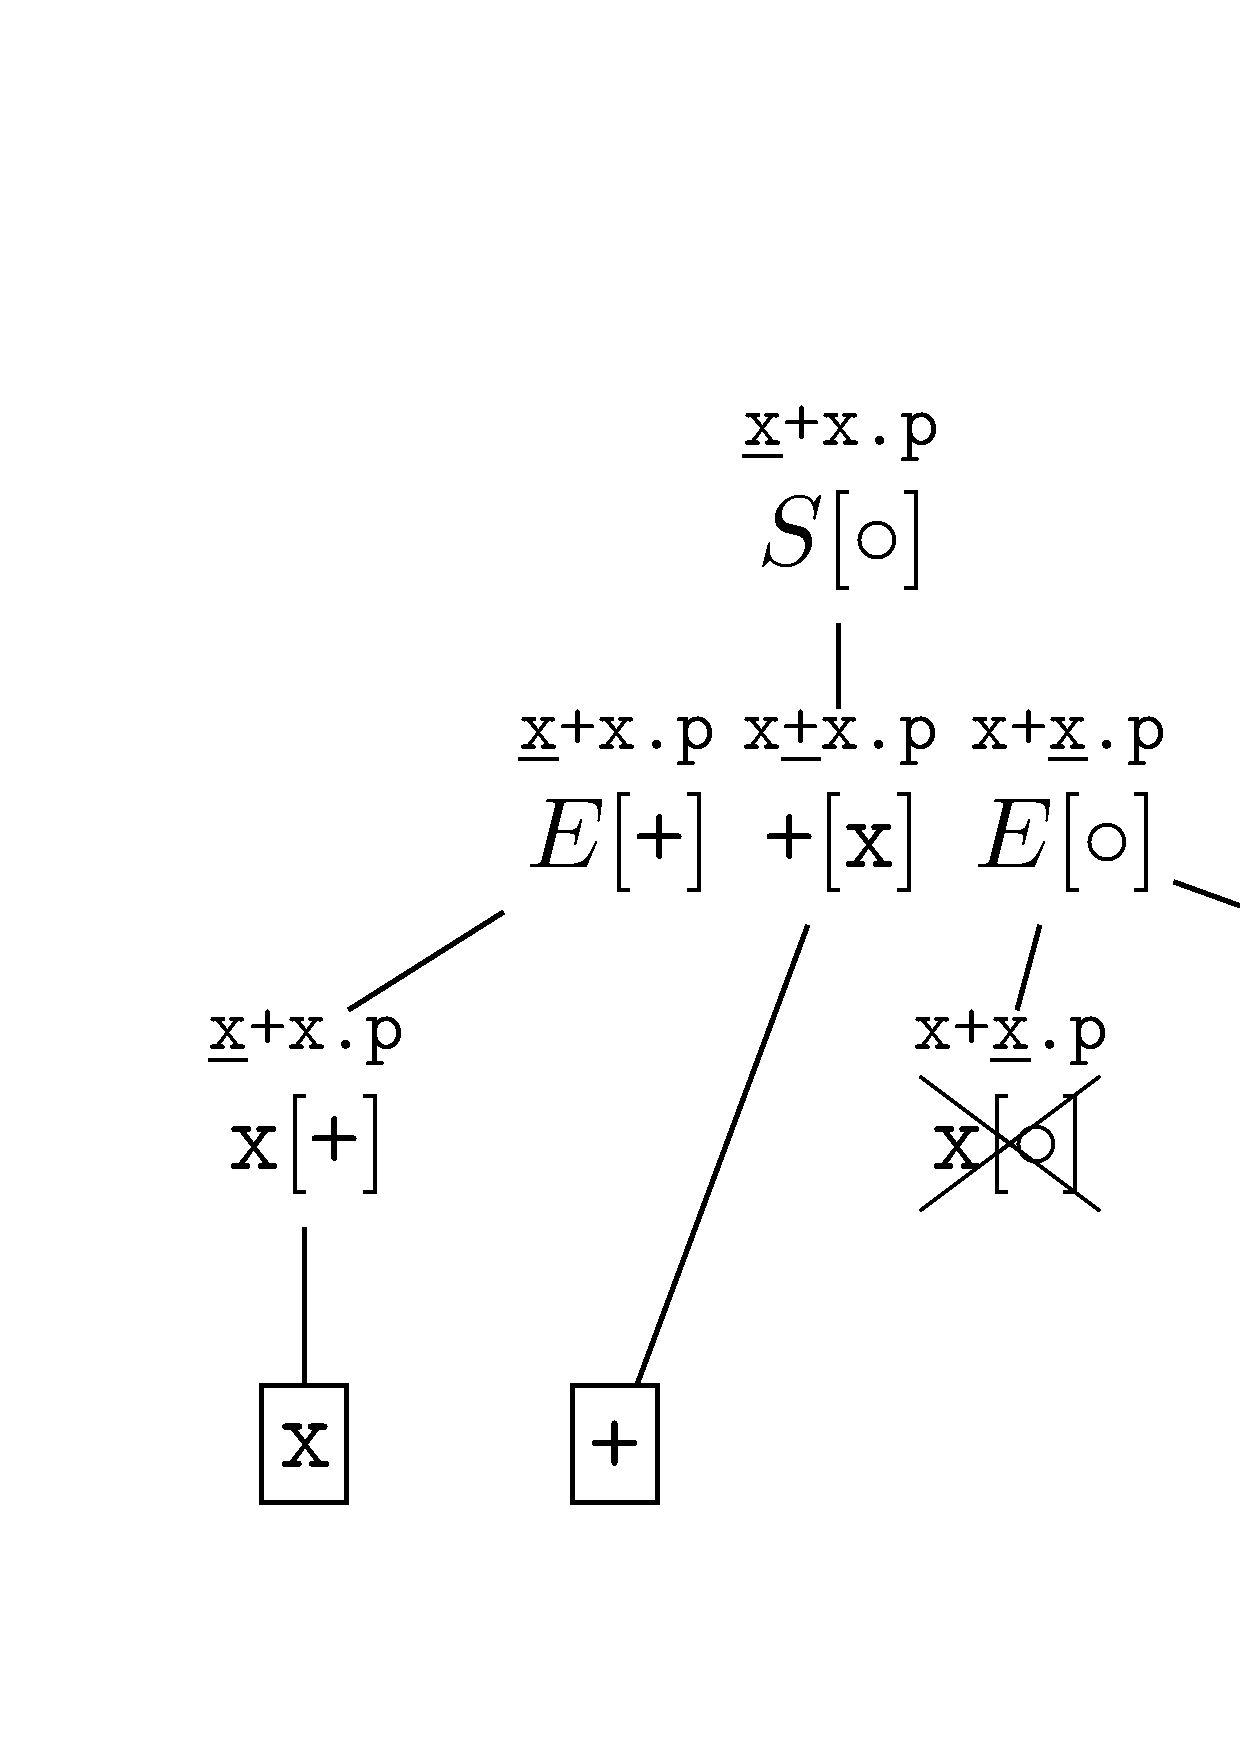
\includegraphics[width=0.33\textwidth]{img/laparser.pdf}
\end{center}

\smallskip
\noindent
Each node \( \symb[\la] \) denotes a symbol \( \symb \) with a set of lookahead
tokens \( \la \).  The underlined character in the string of each node denotes
the current position in the parsing process that follows a pre-order traversal.
The parser starts from the starting non-terminal \( \NT{S} \) with the special lookahead \(
\emptyfirst \), which denotes the end of inputs.  Then, it visits the first
alternative \( \NT{E}~\T{+}~\NT{E} \) with the same lookahead \( \emptyfirst \).
Each symbol is visited with its corresponding lookahead, which is the first
tokens of the right next symbol.  For example, for the second symbol \( \T{+} \)
in \( \NT{E}~\T{+}~\NT{E} \), the next symbol is \( \NT{E} \) and its first
tokens are:
\[
  \begin{array}{r@{~}c@{~}l}
    \symbfirst{\NT{E}} &=& \rhsfirst{\T{x}} \cup \rhsfirst{\T{x.p}}\\
                       &=& \symbfirst{\T{x}} \cup (\symbfirst{\T{x}} \firstplus
    \rhsfirst{\T{.p}}) = \{ \T{x} \}\\
  \end{array}
\]
Thus, the parser visits \( \T{+} \) with the lookahead \( \T{x} \).
The most important point here is the difference between two visits of the
non-terminal \( \NT{E} \) in \( \NT{E}~\T{+}~\NT{E} \).  The first visit of \(
\NT{E} \) has the lookahead \( \T{+} \) and the actual next character after
matching \( \T{x} \) is also \( \T{+} \). Thus, the first alternative \( \T{x}
\) of \( \NT{E} \) is chosen for the first visit.  However, in the second visit
of \( \NT{E} \), the lookahead is the end of inputs \( \emptyfirst \) but the
next character after matching \( \T{x} \) is the dot character (\( \T{.} \))
instead of the end of inputs.  Therefore, the second alternative \( \T{x.p} \) is
chosen in the second visit and the parser now successfully parses the input \(
\code{x+x.p} \).

We formally define the semantics of lookahead parsers in Figure~\ref{fig:laparser}.
The helper function \( \getlap{\la} \) generates a parser by combining all
tokens in the lookahead \( \la \) using prioritized choices.
In this case, the order does not change the semantics of lookahead parsers
because \( \getlap{\la} \) just checks the existence of a given token.

\subsection{Implementation}\label{sec:convert-bnfes}
We implemented the lookahead parsing technique
by extending the Scala parser combinators
library, which is a Scala library for PEG-based parser generation.  We
developed {\sf Parser Generator} to synthesize PEG-based parsers with
lookahead parsing for \( \bnfes \).

\begin{figure}[t]
\centering
\small
\[
  \begin{array}{l@{~}c@{~}l}
    (\symb_1 \cdots \symb_n)[\la] &=&
    \symb_1[\symbfirst{\symb_2 \cdots \symb_n} \firstplus \la] \;
    (\symb_1 \cdots \symb_n)[\la]\\[.1em]
    \epsilon[\la] &=& +\getlap{\la}\\[.1em]
    \T{a}[\la] &=& \T{a} \; +\getlap{\la} \\[.1em]
    \NT{A}(\argument_1, \cdots, \argument_k)[\la] &=&
    \rhs_1[\la] \mid \cdots \mid \rhs_n[\la]\\[.1em]
    && \text{where} \; \NT{A}(\argument_1, \cdots, \argument_k) =
    \rhs_1 \mid \cdots \mid \rhs_n\\[.2em]

    \symb?[\la] &=& \symb[\la] \mid \epsilon[\la]\\[.1em]
    (\pm\symb)[\la] &=& \pm(\symb[\la]) \\[.1em]
    (\symb \butnot \symb')[\la] &=& \symb[\la] \butnot \symb'\\[.1em]
    \nolt &=& \nolt \; +\getlap{\la}
  \end{array}
\]
%\vspace*{-1em}
\caption{Formal semantics of lookahead parsers}
\label{fig:laparser}
\vspace*{-1em}
\end{figure}

\smallskip

\textbf{AST Generation.}
{\sf Parser Generator} first automatically synthesizes ASTs as Scala classes
from a given \( \bnfes \) grammar.  Because the structure of lexical productions do
not affect the ECMAScript semantics, we represent lexical non-terminals as
string values.  For each syntactic production \(
  \NT{A}(\param_1, \cdots, \param_k) ::=
  (\cond_1 \Rightarrow)^? \rhs_1 \mid
  \cdots \mid
  (\cond_n \Rightarrow)^? \rhs_n
\), the generator synthesizes a trait \( \code{A} \) and its multiple
subclasses \( \code{A}_i \) for \(0 \le i \le n-1\)
that represent its alternatives.  Each class \( \code{A}_i \) has
non-terminals in its corresponding alternative as its fields.
For instance, the \( ArrayLiteral \) production in Figure~\ref{fig:array-literal}
gets automatically translated to the following Scala classes:
\begin{lstlisting}[style=smallScalastyle]
trait ArrayLiteral extends AST
case class ArrayLiteral0(x1: Option[Elision])
case class ArrayLiteral1(x1: ElementList)
case class ArrayLiteral2(x1: ElementList, x3: Option[Elision])
\end{lstlisting}

\smallskip

\textbf{Parser Generation.}
The next step is to automatically synthesizes parsers for each production in \(
\bnfes \).  We extended Scala parser combinators to support lookahead parsing
and \( \bnfes \) notations. For example, the synthesized parser from the
production \textit{ArrayLiteral} in Figure~\ref{fig:array-literal}(a) is the one
in Figure~\ref{fig:array-literal}(b).  A na\"{i}ve implementation of lookahead
parsing would take exponential time because of backtracking.  To reduce it
to linear time, we applied the memoization technique introduced in
Packrat parsing~\cite{packrat}.  Moreover, we also implemented the
\textit{growing the seed} technique presented by~\citet{packrat-lr} to support
direct and even indirect left recursive productions.  It enables the synthesis
of parsers without changing the structure of each production in \( \bnfes \).

The synthesized parsers also support the automatic semicolon insertion
algorithm, which is one of the most distinctive parsing features in ECMAScript.
We extended our parsing algorithm to keep track of the right-most position that
fails to be parsed in a given input.  In ECMAScript, the token at that position
is defined as an \textit{offending token} and the automatic semicolon insertion
algorithm is defined with such tokens.  The algorithm is simple when we already
have the positions of offending tokens.  Thus, we just manually supported them
by following the rules defined in Section
11.9\footnote{https://www.ecma-international.org/ecma-262/\#sec-automatic-semicolon-insertion}
in ES10.  The automatic semicolon insertion rules rarely change; since
ES5.1 written in 2011, only one sub-rule was added.
